%!TEX root = ../Thesis.tex

\chapter{基于双阈值对比损失函数的敏感目标检索方法}\label{chapter:double_margin}

\section{引言}
在社交媒体上,经常会有用户把枪支等敏感图片上传到自己的主页,这些图片可能助长非法的枪支交易~\cite{Drange2016,MELE2016FacebookBG},也可能引发其他用户的不适,因此某些类型的枪支图片(如机关枪,自动步枪等)需要适当的监管与控制~\cite{Hsu2018Bumble},如果普通用户在社交媒体上展示不能随意购买的枪支,这可能预示着非法的交易。另外,在取证科学上,取证人员有时也需要根据枪支的图片确定枪支的具体品牌与型号,由于枪支类型的繁杂,除非取证人员经过专门的训练,否则很难从庞大的枪支数据库准确找到具体的枪支类型。基于图像检索的任务能够帮助相关人员有效地解决以上问题。只需要使用已经训练好的模型提取图像的特征,然后计算图像特征之间的距离,采用最近邻方法就可以确定具体的枪支类型。

在本章中,我们把枪支图像的精细(fine-grained)检索问题作为敏感目标检索的一个例子来研究,所谓枪支图像的精细检索,详细来说,就是给定一个检索的枪支图像,我们的方法需要从数据库找到和给定图像属于同样精细类别的图片~\cite{Song2016DeepML,Wang2017DeepML}。图像精细检索任务相当困难,因为不同于行人再识别(ReID)~\cite{Zhao2013UnsupervisedSL,Li2014DeepReIDDF} 与人脸识别~\cite{Wen2016ADF,Taigman2014DeepFaceCT} 等任务,图像精细检索任务中使用的图片都是非对齐的(un-aligned)图片,也就是说,在训练和测试过程中使用的图片,其中的物体可能存在不同的大小,可能位于图像不同的位置,并不像人脸或者行人图片一样已经经过检测算法的检测和裁剪,这些都给图像检索任务带来了相当大的挑战。

随着基于卷积神经网络的方法于 2012 年在 ImageNet~\cite{Russakovsky2015ImageNetLS} 图像分类竞赛中取得压倒性的成功~\cite{Krizhevsky2012ImageNetCW},研究者们发现,对已有的网络模型进行端到端的微调能够大幅度刷新卷积神经网络在不同任务上的性能,他们将基于卷积神经网络的方法应用到了物体检测~\cite{Liu2016SSDSS,Redmon2016YouOL,Lin2017FocalLF,Ren2017FasterRT},图像语义分割~\cite{Shelhamer2017FullyCN,Chen2018DeepLabSI,Noh2015LearningDN} 等领域。与此同时,图像检索领域的研究者也开始使用基于卷积神经网络的方法,希望通过对网络的微调提高模型在检索任务上的准确率。其中,Radenovic 等人~\cite{Radenovic2016CNNIR} 使用 Siamese 架构的网络结合对比损失(contrastive loss)函数~\cite{Chopra2005LearningAS,Hadsell2006DimensionalityRB,Han2015MatchNetUF} 来训练整个模型的结构,Gordo 等人~\cite{Gordo2016DeepIR} 则使用了三通道的网络结构结合常用的三元组损失(triplet loss)函数~\cite{Schroff2015FaceNetAU,Wang2014LearningFI,G2016LearningLI,Weinberger2006DistanceML} 用来学习图像的特征。无论是使用两个分支的网络的结构还是使用具有三个分支的网络结构,他们的目的都是希望通过端到端的学习,得到好的网络参数,使得相似图像在特征空间的距离更近,不相似的图片在特征空间距离更远。当然他们得到的实验结果也表明,端到端的训练能够显著提升模型在常用数据库上的检索效果。

基于 Siamese 架构的方法~\cite{Radenovic2016CNNIR,Chopra2005LearningAS,Bell2015LearningVS} 是一种常用的学习特征距离度量的方法,该方法通过输入图像对(image pair)来进行训练,目的在于通过训练,学习到一个好的图像特征嵌入空间(embedding space),在这个空间中,相似图像之间的特征距离较小,不相似图像之间的特征距离较大。然而,该方法有一个比较明显的缺陷,其使用的对比损失函数是非平衡的:在网络的训练过程中,即使相似图像之间的距离已经非常小,使用该损失函数仍然会产生损失。这个损失函数就像加在相似与不相似图像对上的无形的作用力,对于相似图像对(similar image pair,也称为“正样本对”),通过训练,把他们在特征空间的距离拉近,对于不相似图像对(dis-similar image pair,也称为“负样本对”),通过训练,把他们的特征距离在特征空间推远。但是传统的对比损失函数对相似图像对的“牵引力”太强,导致网络在训练的时候过分注重相似图像对,因此网络的检索性能并不是很高。另外已有的方法的另外一个问题是,他们使用的检索数据库~\cite{Philbin2007ObjectRW,Philbin2008LostIQ} 和 ImageNet 数据库在风格上相似,因而在 ImageNet 数据库训练的分类模型能够容易地适应新的数据库。事实上,这些在 ImageNet 上训练得到的模型,如有名的 AlexNet~\cite{Krizhevsky2012ImageNetCW},VGGNet~\cite{Simonyan2014VeryDC},GoogleNet~\cite{Szegedy2015GoingDW},ResNet~\cite{He2016DeepRL} 等,即使不经过微调,直接使用从这些模型的全连接层或者卷积层提取的特征,也能够在上述的数据库上取得非常不错的效果~\cite{Babenko2014NeuralCF,Babenko2015AggregatingLD,Tolias2015ParticularOR},我们在第 \ref{chapter:mfc}~章的实验也说明了这一点。但是对于枪支数据库,由于该数据库上的图片与 ImageNet 图片风格差异巨大,直接使用检索任务训练这些在 ImageNet 上训练得到的模型,效果并不理想,在 \ref{sec:double_margin_exprt}~节实验部分,我们将展示一些实验结果:即使这些分类模型经过检索任务的微调,在枪支数据库上的效果仍然不佳。

为了解决网络训练过程中正样本对与负样本对贡献的损失不平衡的问题,我们提出了基于双阈值对比损失函数的方法。在该方法中,我们分别给相似与不相似图像对设定阈值,因此在模型训练过程中,正负样本对贡献的损失能够更加平衡。在实验过程中,我们通过采样相似与不相似图像对,计算图像之间的特征距离,得到距离的概率分布,然后在此基础上通过实验选出相似与不相似图像对对应的最佳阈值。实验表明,我们的提出的双阈值方法在相同的情况下的检索性能比传统的单阈值方法高出 34.2\% (使用的基础模型为 VGGNet~\cite{Simonyan2014VeryDC})。为了解决原始的 ImageNet 数据库与 Firearm14k 数据库之间差异过大的问题,我们提出了两步训练的策略。具体来说,我们首先在 Firearm14k 上用分类任务来微调原始的模型,然后在此基础上,使用检索任务(双阈值损失函数)来微调得到的模型。这种策略非常有效,进一步提升了模型的检索性能。

本章的结构组织如下:\ref{sec:double_margin_related_work}~节介绍了一些与本章的方法直接相关的工作,\ref{sec:double_margin_method}~节简要回顾单阈值对比损失函数,然后介绍我们提出的基于双阈值对比损失函数的方法,\ref{sec:double_margin_exprt}~节介绍具体的实验结果,包括双阈值与单阈值对比损失方法的结果比较,两步训练策略的效果,阈值的选择对实验结果的影响,最后比较了我们的方法和其他的方法在不同维度下的检索效果。\ref{sec:double_margin_conclusion}~节总结本章的内容。

\section{相关工作}\label{sec:double_margin_related_work}
枪支图像的检索问题之前很少有人研究,Wen 和 Yao~\cite{Wen2005PistolIR} 提出用枪支的轮廓到中心的距离分布来检索相似图片,分布之间的不同用来衡量两个枪支图片的相似度。他们用到的图片背景都比较单一,并且数据库规模很小,大约为 300 张图片。

Babenko 等人~\cite{Babenko2014NeuralCF} 提出使用分类任务微调神经网络,并观察到检索的结果有所提高,他们使用的是交叉熵损失(cross entropy loss),这种损失并不直接针对检索任务,对未知类别泛化能力不强。Arandjelovi{\'c} 等人~\cite{Arandjelovic2016NetVLADCA} 将传统的 VLAD 方法用神经网络来实现,使用三元组损失来优化模型,将模型用在了地点检索任务上。Gordo 等人~\cite{Gordo2016DeepIR} 提出使用三元组损失,并学习针对检索任务的图像的特征嵌入方法,他们同时结合了物体检测中的 ROIPooling 方法~\cite{Ren2017FasterRT} 来提升模型对物体的定位能力,提高模型的性能。Radenvoi{\'c} 等人~\cite{Radenovic2016CNNIR} 则关注于采用 structure from motion 技术,自动从大量图像中产生合适的训练样本对,他们采用了和我们的方法一样的双分支的 Siamese 网络来学习图像特征,发现使用双分支的网络结构能够取得比三分支结构更好的结果。Cao 等人~\cite{Cao2016QuartetnetLF} 使用了和我们的双阈值损失函数相似的方法来处理过图像实例检索问题,他们在实验中采用了更加复杂的网络结构。

\section{基于双阈值对比损失函数的枪支图像检索方法}\label{sec:double_margin_method}

我们的方法使用了卷积神经网络来得到图像在欧式空间的特征,我们使用了 Siamese 网络架构,结合双阈值对比损失函数来学习有区分性的图像特征表达。在训练的时候,我们采用如图~\ref{fig:train_test_arch} 上部分所示的结构,两个网络的参数是共享的,其中 MAC (maximum activiation of convolutions)是由 Tolias 等人~\cite{Tolias2015ParticularOR} 提出的图像特征表达方法,$l_2$ 代表特征的 $l_2$ 归一化。在测试的时候,图片通过测试网络,经过 $l_2$ 归一化,得到最终的特征,要计算两个图像之间的相似度,可以直接使用点积得到。

\subsection{图像特征表达}

我们使用 MAC~\cite{Tolias2015ParticularOR} 方法来得到图像的特征表达。对于一个图像 $I$,我们使用神经网络的最后一层卷积层输出的特征图,该特征图需经过 ReLU 操作,然后对该特征图使用全局最大池化(global max pooling)操作,得到图像的特征。然后,我们对特征进行 $l_2$ 归一化,得到最终的图像特征,该特征维度为 $C$,$C$ 是网络最后一层卷积层输出的通道个数。

这种特征表示方式的优点在于该网络是全卷积形式的,因此可以接受不同大小的图像作为网络的输入,能够保持图像的长宽比。He 等人~\cite{He2014SpatialPP} 以及 Hao 等人~\cite{Hao2017MFCAM} 的文章都指出,保持图像长宽比,能够取得更好的结果,我们在实验中也发现,在训练时保持图片长宽比,测试集上得到的结果比训练时使用固定长宽的方式要高 2\%。

\begin{figure}[!t]
  \centering
  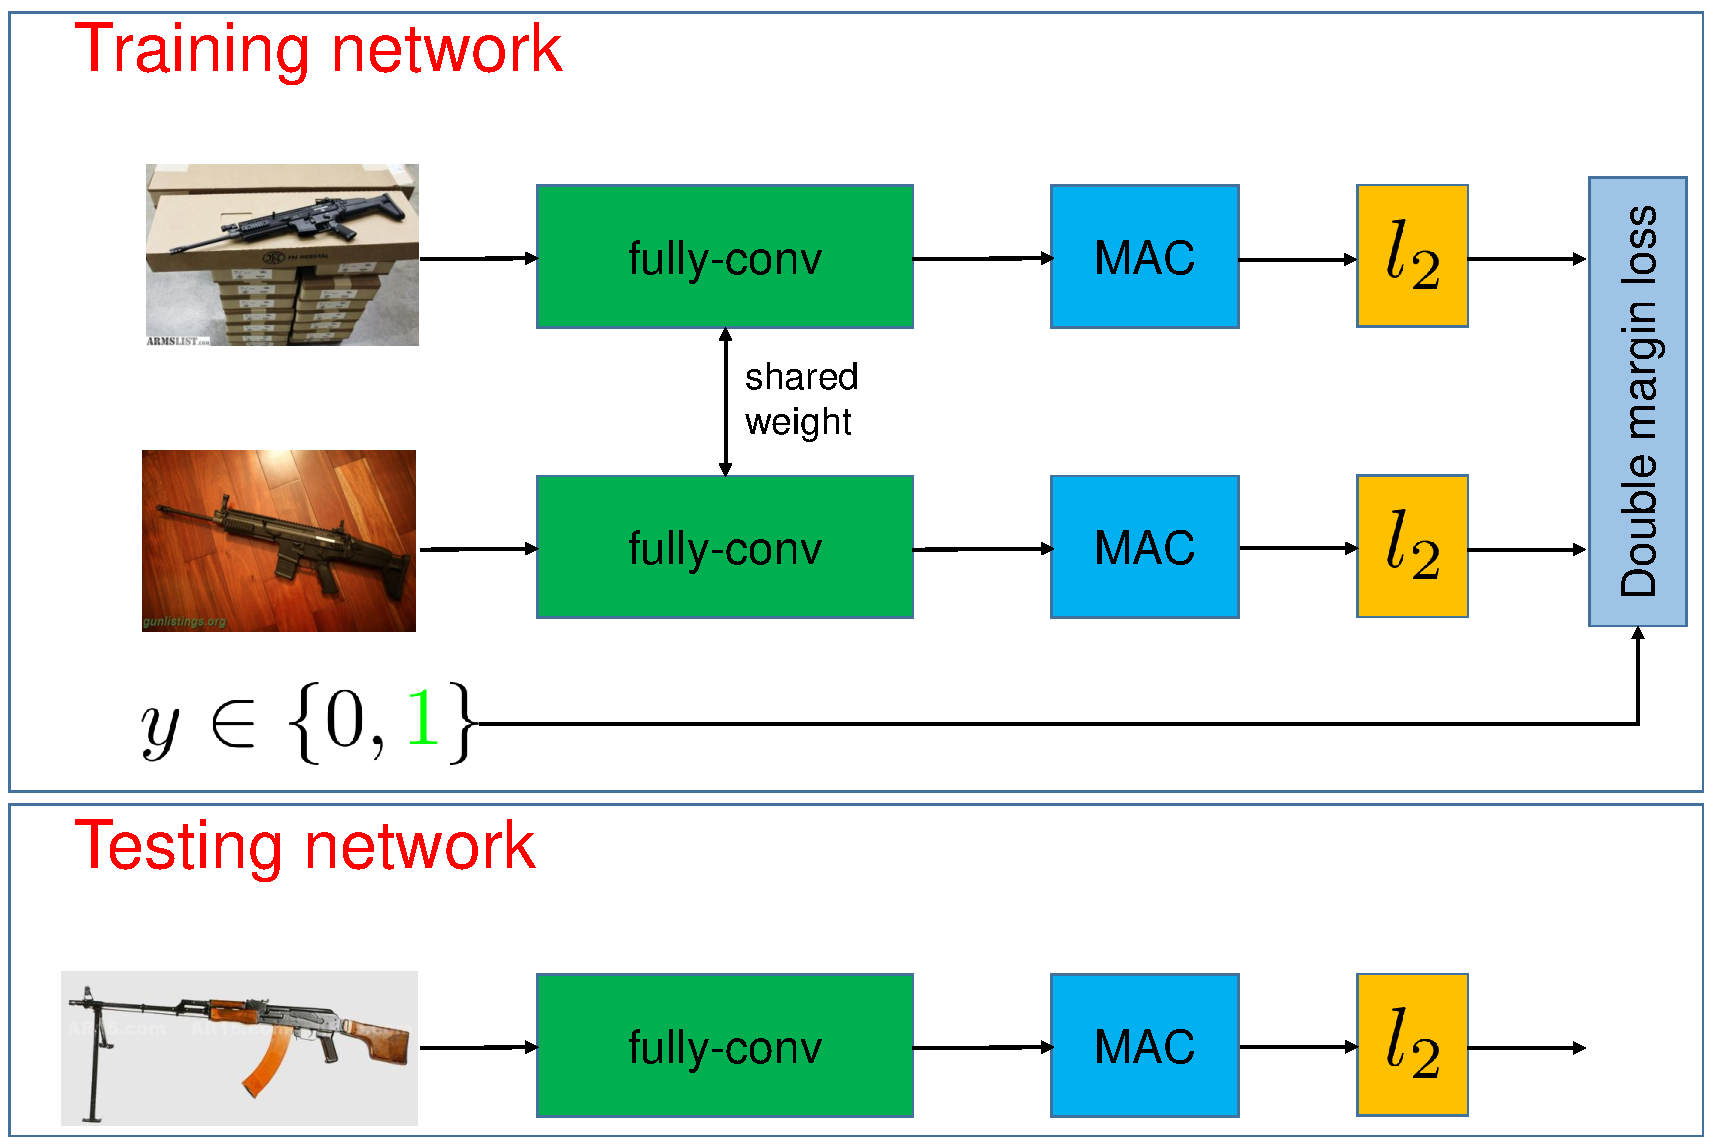
\includegraphics[width=0.95\linewidth]{chapter_double_margin_train_test_arch.pdf}
  \bicaption[基于双阈值对比损失方法的网络结构]{基于双阈值对比损失方法的网络结构,上面为训练网络,下面为测试网络}{The network architecture of the double margin method, \textbf{Top}: training network; \textbf{Bottom}: testing network}
  \label{fig:train_test_arch}
\end{figure}

\subsection{双阈值对比损失函数}
首先我们简要回顾传统的单阈值对比损失函数。给定图像对 $(I_p, I_q)$,以及对应的相似性标签 $y$(如果两张图片是相似的,$y=1$,否则 $y=0$)。假如我们用 $f(I)$ 表示图片 $I$ 经过神经网络得到的特征,那么单阈值对比损失函数可以用如下的公式来表示

\begin{equation}\label{eq:single_margin_loss}
L(I_p, I_q) = \frac{1}{2}\left[yd^2 + (1-y)\max(\alpha - d, 0)^2\right]\, ,
\end{equation}

\noindent上式中,$d$ 是两个图像 $l_2$ 归一化特征之间的欧式距离($d= \lVert f(I_p)-f(I_q)\rVert_2$),$\alpha$ 是对不相似样本设定的一个阈值。单阈值对比损失函数试图把相似图像尽可能拉近,同时把不相似图像之间的距离推的超过设定的阈值 $\alpha$。

单阈值方法的一个明显缺点是网络在训练过程中会偏向相似图片对,因为相似图片对总是会贡献损失,除非相似图片之间的距离为 0。另外一个问题是,在实际训练过程中,很难为不相似图像对设定一个合适的阈值 $\alpha$,使得正负样本对贡献的损失是平衡的。总的来说,这两个问题都导致在实际中很难平衡正负样本贡献的损失,因而不能学习到很好的特征距离度量,导致学习到的模型在 Firearm14k 数据库上检索精度不佳。

为了缓解不平衡的损失问题,我们提出使用双阈值对比损失函数来优化网络模型。该损失函数可以用如下的公式表示

\begin{equation}\label{eq:double_margin_loss}
L(I_p, I_q) = \frac{1}{2}[y\max(d - {\alpha}_1, 0)^2 + (1-y)\max({\alpha}_2 - d, 0)^2]\, ,
\end{equation}

\noindent公式~\ref{eq:double_margin_loss} 中,$\alpha_1$ 和 $\alpha_2$ 是对应于相似与不相似图像对的阈值。很显然,为了使得损失函数有效且有意义,阈值不应该超过两个归一化的特征之间的距离的最大值(为 $\sqrt{2}$),因此下面的不等式成立

\begin{equation}
0 \leq \alpha_1 \leq \alpha_2 \leq \sqrt{2}\, .
\end{equation}

\noindent比较公式~\ref{eq:single_margin_loss} 与 \ref{eq:double_margin_loss},我们可以看出,单阈值与双阈值方法之间的差异主要在于相似图像对的损失如何计算:

\begin{itemize}
\item 单阈值方法:相似图像对总是会贡献损失
\item 双阈值方法:只有两张相似图像的特征距离大于阈值 $\alpha_1$ 的图像对才会贡献损失
\end{itemize}


当我们需要对模型的参数进行小幅度更新以取得更好的结果时,基于双阈值损失函数的方法尤其有效,我们将在实验部分对这种情况下的结果进行说明。我们在实验中发现,由于这种对相似样本更加“缓和”的损失,模型才能在分类任务的基础上继续提高检索的效果,具体实验结果见 \ref{subsec:double_margin_result_analysis}~节。

双阈值对比损失函数(公式~\ref{eq:double_margin_loss})中的两个阈值是该损失函数的核心,我们根据相似与不相似图像对的特征距离的分布来选择这两个阈值。由于数据库中图片数量庞大,可以组成的相似与不相似图像对的数目也十分庞大,因此不可能穷举所有组合,实际上,我们的做法是随机从训练集中采样大约 400000 对图像(相似图像对与不相似图像对的数目相等),并计算图像对特征距离,分别得到相似与不相似图像对特征距离的分布。然后我们把两个分布的均值作为选取两个阈值 $\alpha_1$ 和 $\alpha_2$ 的起点。

\subsection{两步训练策略}

我们在训练中使用的基础模型是从 ImageNet 数据库训练得到的分类模型,由于 ImageNet 数据库和我们的 Firearm14k 数据库差异非常大,Firearm14k 图像的特征不能很好地被基础模型所表达。为了解决这个问题,我们首先使用分类任务微调基础模型,经过分类任务微调以后,模型已经能够比较好地表达 Firearm14k 数据库中的图像特征,此时的检索性能已经较好。然后,在分类微调后模型的基础上,进一步使用我们提出的双阈值损失函数对模型进行微调,实验表明,检索的结果会得到进一步的提升。

\subsection{特征降维}
当训练过程完成以后,我们进一步使用主成份分析法(PCA)对特征进行降维,因为 PCA 能够进一步提升特征的效果~\cite{Radenovic2016CNNIR,Babenko2014NeuralCF,Tolias2015ParticularOR,Babenko2015AggregatingLD}。在我们的实验中,我们使用了 PCA 方法,但是并未使用白化 (whitening),因为我们发现白化操作会引起检索效果的大幅度下降。

\section{实验}\label{sec:double_margin_exprt}
\subsection{评价指标}
在实验中,我们在训练集上训练模型,在验证集上采用 mAP 来选择合适的模型。我们使用两种评价指标来报告模型在测试集上的结果。第一种评价指标是 mean average precision (mAP),mAP 常用来衡量检索系统的总体性能。第二个评价指标是 Rank-k 准确率~\cite{Jgou2011ProductQF,Song2016DeepML},Rank-k 准确率计算的是在所有的查询图片中,其 $K$-邻近图片中存在至少一张同类图片的查询图片的比例。Rank-k 准确率注重于检索方法返回的 top-k 的结果,在实际场景下,如图像搜索引擎及电商网站在线购物,用户更关心前面返回 $K$ 个结果,因此 Rank-k 准确率这个指标更加能够反映实际需求。

\subsection{实验设置}
我们使用了开源深度学习框架 PyTorch\footnote{\url{http://pytorch.org/}} 来实现我们的整个方法,我们使用的服务器搭载了英伟达 TITAN X(Pascal) GPU,显存容量为 12G,同时搭载两颗英特尔 Xeon 12 核 CPU。在实验中,我们所用的基础模型为 VGG16 模型~\cite{Simonyan2014VeryDC},该模型是在 ImageNet 分类数据库上训练得到的。针对我们的任务,我们对模型进行了一些修改,我们把模型的全连接部分去掉,只使用了该模型的全卷积部分。

我们使用了两步训练的办法对模型进行了训练,下面分别介绍这两步训练的过程。

\begin{enumerate}
\item 使用分类损失微调网络

在这个步骤中,我们使用了 Firearm14k 数据库中的训练集和验证集的所有 127 类图片,我们把这些图片分为训练和验证数据,比例为 70\% 和 30\%。我们在第 \ref{chapter:firearm_dataset}~章 \ref{sec:dataset_stats}~节已经提到过,该数据库类别高度不平衡,因此我们使用了加权的交叉熵损失函数来训练网络,对于某个样本来说,该损失函数形式如下:

\begin{equation}
l = -w_k \log\frac{\exp(x_k)}{\sum_{i=0}^{126} \exp(x_i)}
\end{equation}

\noindent上式中,$k$ 是该样本的真实类别,神经网络的输出为 127 个节点,$x_i$ 是神经网络在第 $i$ 个节点的输出值,$w_k$ 是第 $k$ 类对应的权重。我们使用的批(batch)大小为 128,训练过程(epoch)数量为 50,初始学习率(learning rate)为 0.001,冲量(momentum)为 0.9,权值衰减(weight decay)系数为 0.0005,学习率每过 30 个训练过程,减为之前的十分之一。

为了防止模型过拟合,我们也使用了数据增广~\cite{Krizhevsky2012ImageNetCW}(data augmentation),由于我们使用的网络可以接受不同大小的图像,因此我们在实验中保持图像长宽比不变,把图像的最长边缩放到 $[256, 384]$ 这个范围 (步长为 8),同时我们也使用了随机的水平翻转,旋转以及颜色变换(亮度,对比度等变化)。基础网络的分类微调过程,大约耗时 2 个小时。最后,我们选择在验证数据上分类准确率最高的模型,然后在这个模型基础上再进行第二步的训练。

\item 使用双阈值对比损失函数微调网络

正如 \ref{sec:double_margin_method}~节介绍的,使用 Siamese 结构的网络训练图像时,需要输入一对图像以及相应的标签,因此我们需要生成训练数据。对于 Firearm14k 训练集中的每一类图像,我们随机生成 180 对相似图像对以及 180 对不相似图像对。我们总共生成了 38520 对图像来训练第一步得到的网络模型。当然,对于神经网络来说,这样的训练数据量并不够,为了增加图像的多样性,增强模型的泛化能力,每 5 个训练过程,我们会重新生成一次训练图像对。在训练过程中,我们同样使用了数据增广方法,和分类训练数据增广方法一致,这里不再赘述。

由于输入网络的图像大小以及长宽比不同,我们无法使用传统的批处理(batch processing)的方法来输入图像,在训练过程中,我们每次输入一个图像对,然后反传误差,等输入网络的图像对达到 64 对时\footnote{所以可以认为我们使用的批大小是 64},我们对网络的参数进行一次更新。在验证集上,我们使用 mAP 衡量网络的性能,从而选择最佳的网络模型。我们使用随机梯度下降方法优化网络的参数,实验中使用的参数设置为:初始学习率为 0.001(每过 10 个训练过程变为原来的十分之一),冲量为 0.9,权值衰减为 0.0005。网络的最大训练过程为 30,整个训练大约需要 14 个小时的时间。
\end{enumerate}

\subsection{实验结果与分析}\label{subsec:double_margin_result_analysis}

本节介绍具体的实验,主要有单阈值与双阈值对比损失函数的比较与结果分析,两步训练的结果以及分析,以及双阈值函数中的两个阈值选取对检索性能的影响分析。

\begin{table}[t]
  \centering
  \bicaption{单阈值方法与双阈值方法的对比}{Comparison between the single margin and double margin contrastive loss}
  \label{table:single_vs_double}
  \begin{tabular}{@{}lllllll@{}}
    \toprule
    \multirow{2}*{} & \multirow{2}*{方法} & \multirow{2}*{mAP(\%)} & \multicolumn{4}{c}{Rank-k 准确率(\%)} \\

    \cmidrule(lr){4-7}
    & & & k=1 & k=2 & k=4 & k=8 \\
    \midrule
    (a) & VGG  & 31.1 & 83.75 & 91.25 & 95.0 & 96.25 \\
    \midrule
    (b1) & retr-s & 35.1 & 80.0 & 86.25 &  92.5&  96.25\\
    (b2) & retr-d & 47.1 & 87.5 & 88.75 & 95.0 & 97.5 \\
    \bottomrule
  \end{tabular}
\end{table}

\noindent\textbf{(1)单阈值与双阈值对比损失函数的比较}

在本部分,我们评估了所提出的双阈值对比损失函数的有效性,和单阈值对比损失函数进行了比较。在我们的比较中,双阈值与单阈值方法使用了相同的基础模型(VGG16 模型)并且使用了相同的设置。对于两种方法,我们都进行了多轮实验,然后我们从多轮实验中选择效果最好的模型来比较这两个方法。我们在表~\ref{table:single_vs_double} 列出了两种方法在测试集上的实验结果,对于 Rank-k 准确率,我们使用了 $k=[1,2,4,8]$。在表~\ref{table:single_vs_double} 中,第一行“VGG”是使用原始 VGG 网络得到的结果,第二行“retr-s”代表使用单阈值对比损失函数得到的检索结果,第三行“retr-d”代表使用双阈值损失函数得到的结果。从这些结果,我们可以看出:

\begin{itemize}
\item 单阈值与双阈值方法都可以提高基础的 VGG 模型的 mAP。
\item 原始的 VGG 的模型已经在 Rank-k 准确率这个指标上取得了不错的效果,因而 Rank-k 准确率这个指标更加具有挑战性。基于双阈值损失函数的方法在这个指标上仍然有所提高,但是基于单阈值损失函数的方法在这个指标上反而比原始的 VGG 模型还要差。
\end{itemize}
\begin{figure}[t]
  \centering
  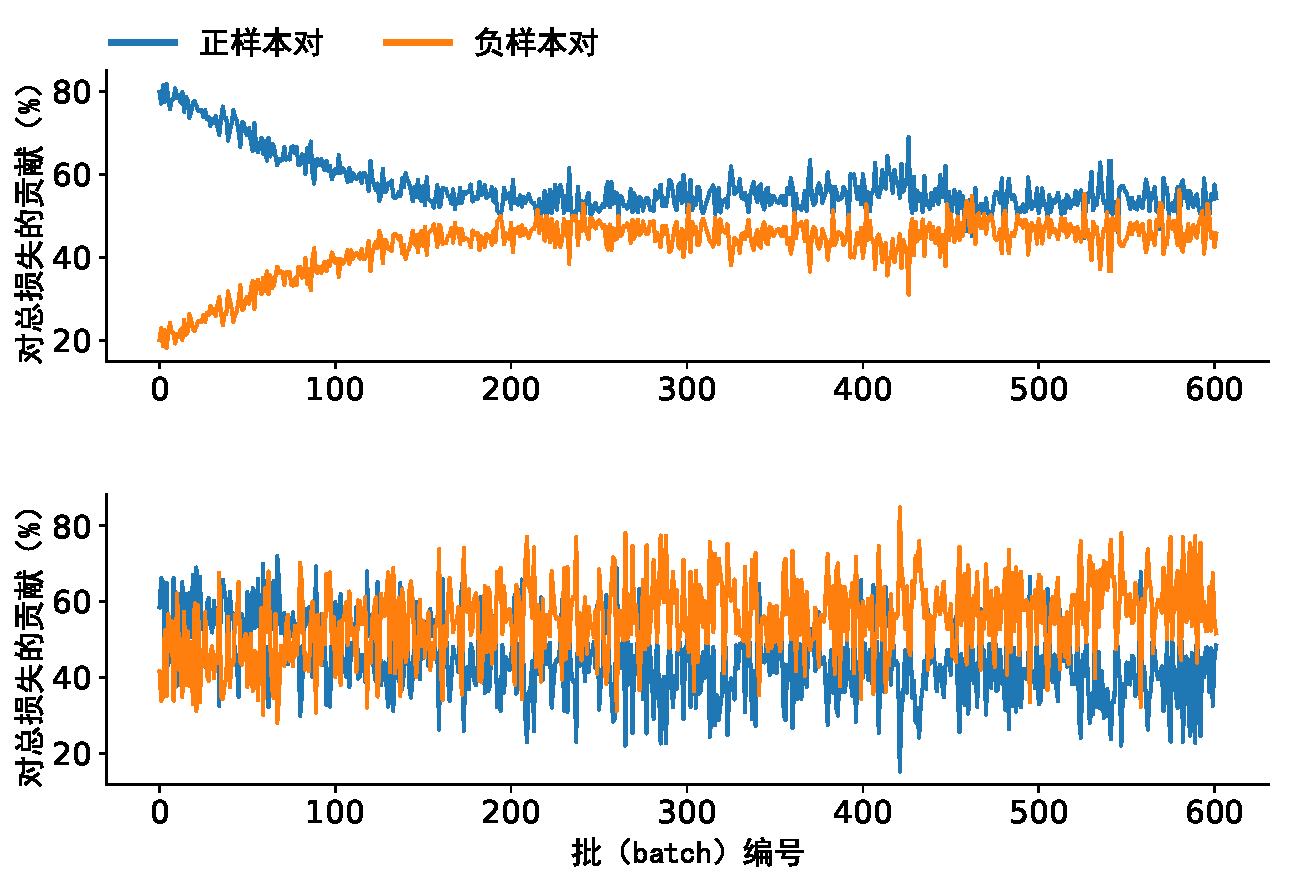
\includegraphics[width=0.95\linewidth]{chapter_double_margin_pos_neg_loss_contrib.pdf}
  \bicaption[使用不同损失函数时,正负样本对对损失的贡献率]{使用不同损失函数(\textbf{上图}:单阈值对比损失函数,\textbf{下图}:双阈值对比损失函数),一个训练过程中不同批次数据,相似样本对与不相似样本对对总体损失的贡献率}{The contribution of positive pairs and negative pairs to the total loss in a training epoch using different loss fuctions (\textbf{Top}: single margin contrastive loss; \textbf{Bottom}: double margin contrastive loss)}
  \label{fig:img_pair_loss_contribution}
\end{figure}

总的来说,基于双阈值对比损失函数的方法在两种评价指标下的效果都优于传统的单阈值损失函数,双阈值损失函数在 mAP 指标上取得了 47.1\% 的结果,而单阈值方法只取得了 35.1\% 的结果,双阈值方法相对于单阈值方法整整提高了 34.2\% 的 mAP,而且没有额外的时间和内存等开销,这说明了双阈值损失函数的有效性。

我们也从直观上研究了为什么基于双阈值损失函数的方法更加有效。我们分别画出了基于双阈值函数的方法以及基于单阈值函数的方法,在一个训练过程中不同批数据中,相似样本对以及不相似样本对对整个损失的贡献率,所得到的结果如图~\ref{fig:img_pair_loss_contribution} 所示。图~\ref{fig:img_pair_loss_contribution} 上部分展示的是使用单阈值对比损失函数的结果,下部分展示的使用双阈值对比损失函数的结果。可以看出,使用单阈值损失函数时,刚开始训练时的一些批次数据,正样本对对总的损失的贡献明显大于负样本对,这样的话,网络的训练可能会被引入错误的方向,导致后续模型优化出现方向错误,因而检索效果很差;使用双阈值损失函数,从训练一开始,正样本贡献的损失与负样本贡献的损失相对平衡,因而网络优化方向更好,检索的效果也更好。

\begin{table}[t]
\centering
 \bicaption{两步训练策略的结果}{The result of two-step training strategy}
 \label{table:two_step_training}
	\begin{tabular}{@{}lllllll@{}}
		\toprule
		\multirow{2}*{} & \multirow{2}*{方法} & \multirow{2}*{mAP(\%)} & \multicolumn{4}{c}{Rank-k 准确率(\%)} \\

		\cmidrule(lr){4-7}
		& & & k=1 & k=2 & k=4 & k=8 \\
		\midrule
		(a) & VGG  & 31.1 & 83.75 & 91.25 & 95.0 & 96.25 \\
		\midrule
		(b1) & Cls & 65.4 & 92.5 & 96.25 & 97.5 & 98.75 \\
		(b2) & Cls + retr-s & -- & -- & -- & -- & -- \\
		(b3) & Cls + retr-d &  68.4 & 95.0 & 98.75 &98.75 & 100.0 \\
		\bottomrule
	\end{tabular}
\end{table}

\noindent\textbf{(2)两步训练策略的效果}

我们进一步研究了两步训练策略的有效性。首先我们使用分类任务(采用加权的交叉熵损失)来微调网络的参数,然后我们在分类微调得到的模型基础上,再使用双阈值对比损失函数进行优化。我们将实验的结果列在表~\ref{table:two_step_training} 中,“Cls”表示使用分类任务训练得到的结果,“Cls + retr-s”代表先使用分类任务后使用单阈值损失函数得到的结果,“Cls + retr-d”代表先使用分类任务后使用双阈值损失函数得到的结果。

从实验结果,我们可以看出,仅仅通过在分类任务上训练模型,在 mAP 这个指标上,我们得到的模型相对于基础的 VGG 模型已经取得了 110.2\% 的效果增强。我们发现,在分类微调的模型基础上,在使用单阈值对比损失函数无法进一步提高模型的检索效果,但是使用双阈值对比损失函数微调模型,无论在 mAP 还是 Rank-k 准确率的指标上都可以进一步提高网络的检索效果。实际上,我们发现,如果使用单阈值方法,无论我们设定阈值为多少,随着训练过程的进行,模型的性能会持续下降(因此在表~\ref{table:two_step_training} 中,我们没有列出“Cls + retr-s”的结果)。这种情况是可以预见的:因为模型经过分类任务的微调,当我们再使用检索任务微调模型的参数时,必须要小心,使用单阈值的方法将会使得模型优化向错误的方向前进(因为单阈值方法中,相似图像对的损失占上风)。正是由于使用双阈值损失函数,正负样本贡献的损失更加平衡,所以模型的检索效果得到进一步提升。

\begin{figure}[t]
	\centering
  \captionsetup{justification=centering}
	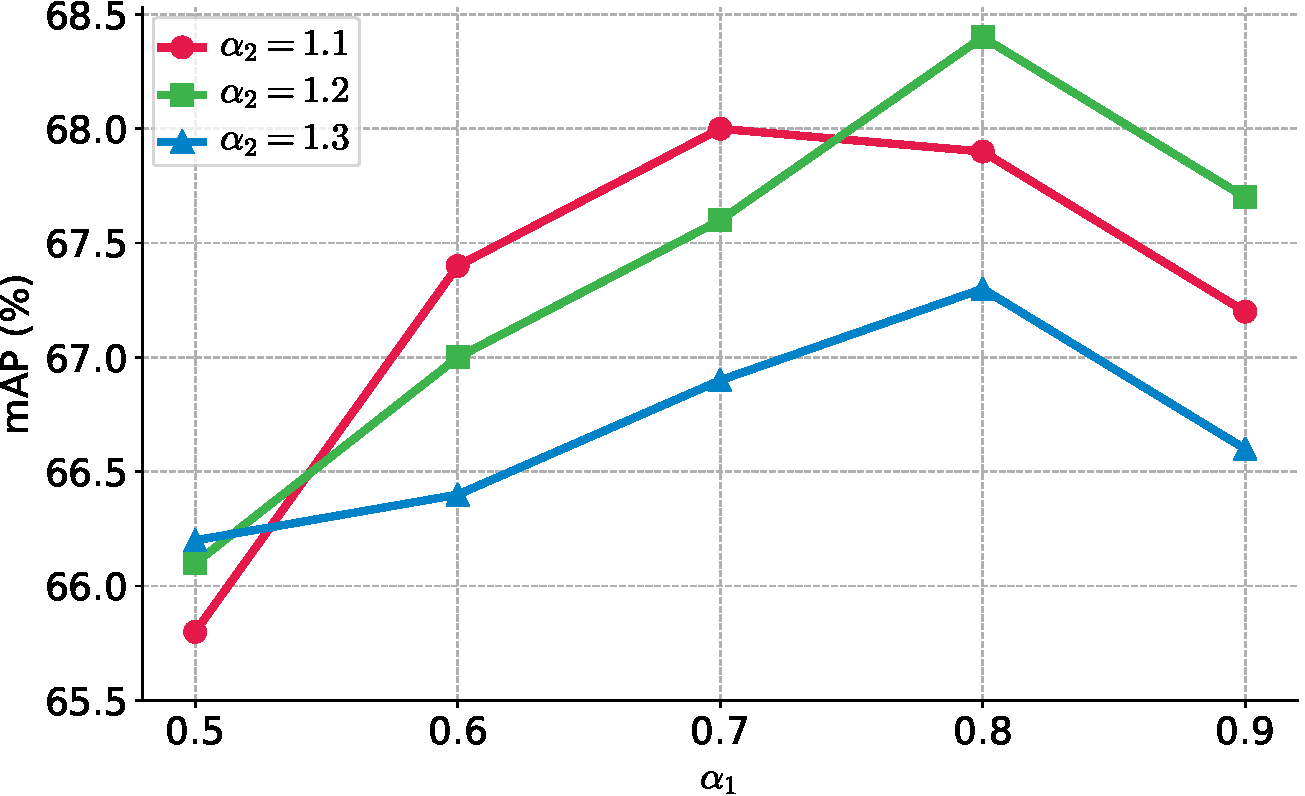
\includegraphics[width=\linewidth]{chapter_double_margin_impact_of_margins.pdf}
	\bicaption{双阈值对比损失函数中两个阈值对模型检索性能的影响}{The impact of the two margin terms in the double margin contrastive loss on the retrieval performance of the model}
	\label{fig:impact_of_margins}
\end{figure}

\noindent\textbf{(3)阈值选取及对检索结果的影响}

在本部分,我们将讨论双阈值损失函数中的两个阈值 $\alpha_1$,$\alpha_2$ 对模型检索效果的影响。正如在 \ref{sec:double_margin_method} 节讨论的那样,我们使用在分类任务上微调好的模型(因为检索的模型是在分类模型的基础上进行优化的),从训练数据库采样图像对,然后计算图像对中两幅图像的特征之间的距离,然后画出相似图像对与不相似图像对特征距离的分布曲线。这两个分布曲线近似为正态分布,具体例子可以参见图~\ref{fig:feat_dist_distribution_change} 中的某一张图。我们把两个分布的均值作为阈值选择的起点,对于相似和不相似图像对,两个分布均值分别为 0.9 以及 1.2。图~\ref{fig:impact_of_margins} 展示了两个阈值对模型检索性能的影响(以 mAP 指标来衡量)。从图上可以看出,两个阈值的选取应该在分布的均值附近选择,才能取得比较高的检索结果,另外,两个阈值之间的间隔非常重要,这个间隔不能太“松弛”(也就是说 $\alpha_2 - \alpha_1$ 太小),也不能太“紧”($\alpha_2 - \alpha_1$ 太大),无论间隔太大或者太小,都会影响模型的性能。最终,我们选择设定 $\alpha_1=0.8$ 以及 $\alpha_2=1.2$ 来优化我们的模型。

\begin{figure}[t]
	\centering
  \captionsetup{justification=centering}
	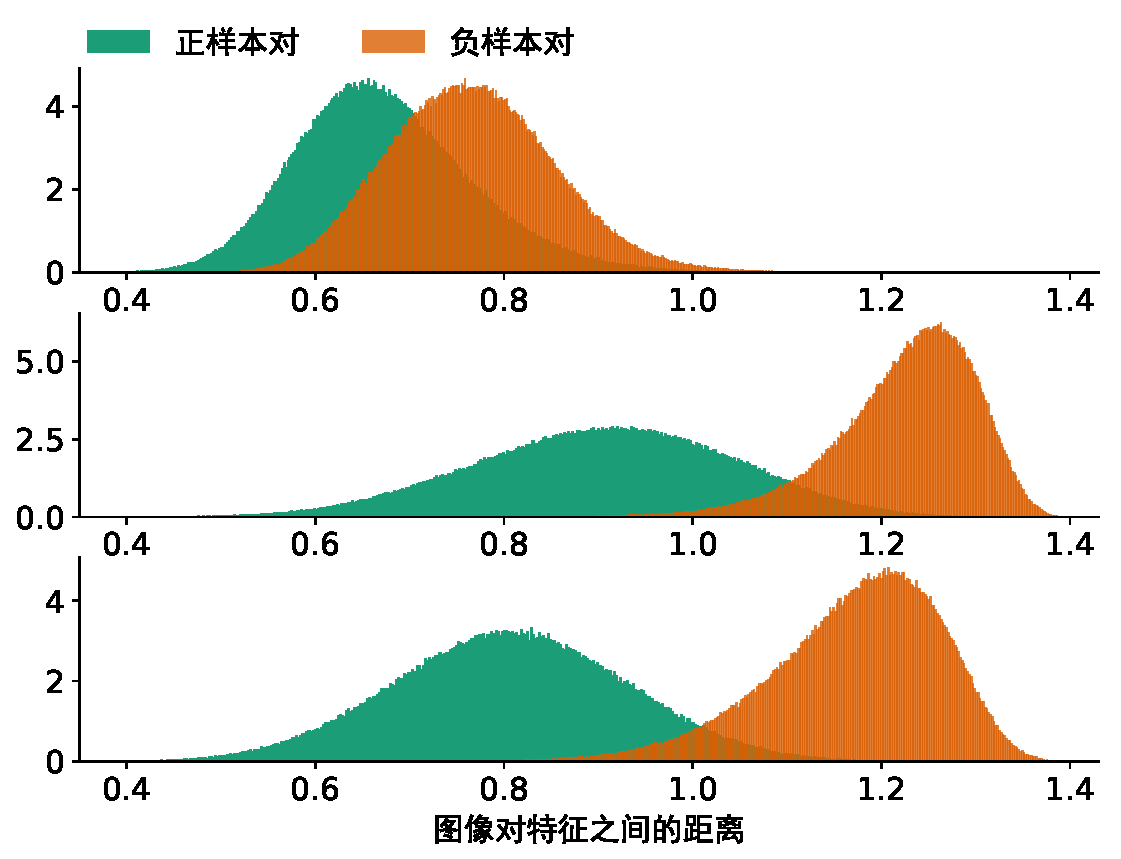
\includegraphics[width=\linewidth]{chapter_double_margin_dist_distribution_change.pdf}
	\bicaption{不同模型下相似与不相似图像对特征距离的概率分布}{The feature distance probability distributions of positive and negative pairs under different models}
	\label{fig:feat_dist_distribution_change}
\end{figure}

\subsection{检索效果的可视化}
在本部分,我们将采用可视化的方式来帮助我们理解为什么所提出的方法能够取得更好的效果。我们比较了三种不同的模型,第一种是原始的 VGG16 模型,第二种是在 Firearm14k 数据库使用分类任务微调以后的模型,第三种是在分类模型基础上继续使用双阈值损失函数微调的得到的模型。我们随机采样了大约 500000 相似与不相似图像对,然后我们分别使用了不同模型计算相似与不相似图像对特征距离。图~\ref{fig:feat_dist_distribution_change} 展示了不同模型下,正负样本对特征距离的分布曲线。对于原来的 VGG 模型(图~\ref{fig:feat_dist_distribution_change},\textbf{上图}),相似图像对与不相似图像对的图像特征距离分布重合非常大,因此模型输出的特征对于判断两个图像是否是相似有很大的不确定性,所以检索结果较差(31.1\% mAP)。经过在分类任务上的微调,我们得到了第二个模型(图~\ref{fig:feat_dist_distribution_change},\textbf{中图}),相似与不相似图像对的特征距离分布之间的重叠大幅减少,因此模型的检索精度也有了很大的提升(检索的 mAP 为 65.4\%)。当我们进一步在分类模型基础上使用双阈值损失函数对模型进行微调后,我们得到了最终的模型(图~\ref{fig:feat_dist_distribution_change},\textbf{下图}),我们可以看到特别是相似图像对的特征距离分布发生了明显的变化:分布曲线的形状发生了变化,相对于中图的“矮胖”,变得更加“高瘦”。分布的变化也带来了检索结果的进一步提升(检索 mAP 68.4\%)。在图~\ref{fig:double_margin_retrieval_result} 中,我们也展示了一些采用我们的方法得到的检索结果,从这些结果我们可以看出,当枪支图片只占据图像的一小部分时候,我们的方法可以准确找到相似的图片(例如,第 2 个和第 7 个检索结果),另外我们的方法对于枪支的姿态、角度变化也具有较强的鲁棒性。

\begin{figure}[t]
	\centering
	\includegraphics[width=\linewidth]{chapter_double_margin_retrieved_results_more.pdf}
	\bicaption{我们的方法的一些示例检索结果}{Some of the retrival results using our proposed method}
	\label{fig:double_margin_retrieval_result}
\end{figure}


\begin{figure}[t]
	\centering
	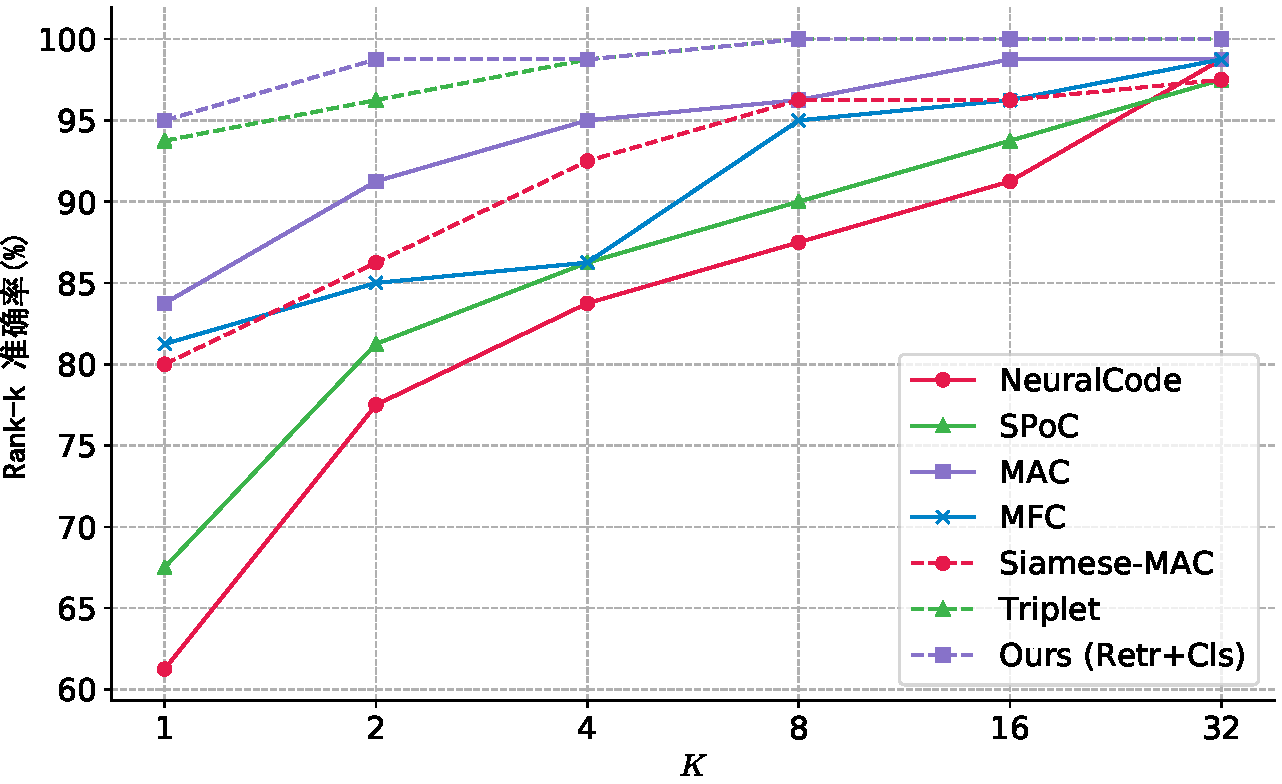
\includegraphics[width=\linewidth]{chapter_double_margin_compare_rank_k_accu.pdf}
	\bicaption{不同方法 Rank-k 准确率的比较(\%)}{Comparison of Rank-k accuracy between different methods}
	\label{fig:rank_k_accuracy_compare}
\end{figure}

\begin{table}[!t]
  \centering
  \begin{threeparttable}
    \bicaption{与其他主流方法的结果比较}{Comparison with the state of the art methods}
  \label{table:firearm_retrieval_compare_with_soa}
  \begin{tabular}{@{}lllllll@{}}
    \toprule
   \multirow{2}*{方法} & \multicolumn{6}{c}{特征维度}\\
    \cmidrule(lr){2-7}
     & D=512 & D=256 & D=128 & D=64 & D=32 & D=16\\
    \midrule
    Neural codes~\cite{Babenko2014NeuralCF} & 15.9 & 15.8 & 15.7 & 14.6 & 13.7 & 10.5\\
    SPoC~\cite{Babenko2015AggregatingLD} & 23.3 & 23.4 & 23.1 & 22.4 & 20.6 & 18.4\\
    MFC~\cite{Hao2017MFCAM} & 30.0 & 29.8 & 29.5 & 28.0 & 24.5 & 20.9 \\
    MAC~\cite{Tolias2015ParticularOR} & 36.1 & 36.4 & 36.5 & 35.4  & 32.3 & 27.8\\
    \midrule
    Siamese-MAC~\cite{Radenovic2016CNNIR} & 35.6 & 36.2 & 37.2 & 37.3 & 35.2 & 31.4\\
    TripletNet\textsuperscript{$\dagger$}~\cite{Gordo2016DeepIR} & 67.98 & 68.57 & 69.60 & 69.97 & 68.1 & 60.67\\
    \midrule
    Ours (retr-d) & 45.79 & 46.17 & 46.61 & 46.75 &45.36 & 42.03 \\
    Ours (cls) & 66.57 & 67.2 & 68.53 & 68.67 & 67.47 & 59.99\\
    Ours best (cls + retr-d) & \textbf{68.63} & \textbf{69.15} & \textbf{70.14} & \textbf{70.07} & \textbf{68.48} & \textbf{61.59}\\
    \bottomrule
  \end{tabular}
  \begin{tablenotes}
      \footnotesize
      \item \textsuperscript{$\dagger$} TripletNet 的权重是也由 Firearm14k 分类微调的模型初始化的。
  \end{tablenotes}
  \end{threeparttable}
\end{table}

\subsection{与其他方法的对比}
在本节,我们比较了所提出的双阈值方法与其他主流方法的检索结果,这些方法中,有的方法使用的是未经过微调的模型(称为 off-the-shelf 模型),另外一些方法使用的是经过微调的模型。为了保证对比的公平性,所有的方法都由我们使用 VGG16 模型实现。对于那些基于 off-the-shelf 模型的方法~\cite{Babenko2014NeuralCF,Tolias2015ParticularOR,Babenko2015AggregatingLD,Hao2017MFCAM},我们根据论文中所给的设置来实现对应的方法,在这些方法中,MFC 是我们在第 \ref{chapter:mfc}~章提出的多尺度全卷积的方法。对于那些使用模型微调的方法~\cite{Gordo2016DeepIR,Radenovic2016CNNIR},我们使用了和我们的方法尽可能一致的设置,然后在 Firearm14k 数据库上训练模型。按照惯例~\cite{Babenko2015AggregatingLD,Radenovic2016CNNIR},从这些方法得到的图像特征都经过 $l_2$ 归一化,然后经过了 PCA 变换,最后再一次经过 $l_2$ 归一化处理。

首先,我们报告不同的方法在 mAP 指标上的结果,所有的实验结果参见表~\ref{table:firearm_retrieval_compare_with_soa}。这里的结果表明,off-the-shelf 模型(表~\ref{table:firearm_retrieval_compare_with_soa},\textbf{上部})的 mAP 分数都相对较低,这是由于 Firearm14k 数据库和 ImageNet 数据库的巨大差异,这些预训练的模型无法生成具有区分性的特征,因而检索效果并不理想。使用单阈值方法微调的模型~\cite{Radenovic2016CNNIR} 表现也不理想,使用三元组损失的 TripletNet~\cite{Gordo2016DeepIR} 的表现相对单阈值方法提高了很多。最后,我们的提出的方法在不同的特征维度下都超过了其他方法。值得注意的是,我们的方法在特征维度被压缩到极低的情况下仍然表现良好,例如当特征维度为 16 时,检索的 mAP 仍然达到了 61.59\%。

我们也计算了不同方法在 Firearm14k 测试集上的 Rank-k 准确率,在这个实验中,我们使用的是 512 维特征,得到的实验结果如图~\ref{fig:rank_k_accuracy_compare} 所示。从图中可以看出,当 $k$ 比较大时($k=16$ 或 $k=32$ 时),各种方法的 Rank-k 准确率都较高,这说明 Rank-k 指标是比较容易的指标;当 $k$ 比较小时,SPoC~\cite{Babenko2015AggregatingLD},NeuralCode~\cite{Babenko2014NeuralCF} 和 Siamese-MAC~\cite{Radenovic2016CNNIR} 等方法,表现较差,TripletNet 方法~\cite{Gordo2016DeepIR} 和我们的方法此时表现较好,特别是我们的方法,在 $k=1$ 或 $k=2$ 时,表现要优于 TripletNet 方法。

\section{本章小结}\label{sec:double_margin_conclusion}
在本章中,我们详细介绍了提出的双阈值对比损失函数,提出该方法的动机主要有两个,一是目前单阈值对比损失函数无法保证正负图像对在训练时贡献的损失的平衡,二是我们提出的 Firearm14k 数据库与 ImageNet 数据库之间的巨大差异导致直接微调模型效果欠佳。我们提出使用双阈值对比损失函数来解决模型训练过程中正负图像对贡献的损失不平衡的问题,同时提出使用两步训练的策略来解决数据库之间图像差异大的问题。在实验部分,我们把提出的方法与当前的主流方法进行了比较,并给出可视化的分析,证明我们的方法为什么有效,实验结果表明我们的方法在不同的特征维度下检索效果都超过了当前的主流方法。指的说明的是,虽然我们是在枪支图像库进行的实验,我们的方法对于类似的检索问题都是适用的。
